\section{Trigeminal Neuralgia}

Trigeminal neuralgia (TN) is a chronic neuropathic facial pain disorder, that commonly affects one or more branches of the trigeminal nerve. TN symptoms involve paroxysmal, shock-like pain condition affecting one or more of the three facial sensory nerve branches. The pain episodes can be unpredictable, as the length of episodes can range from months to years \cite{Katusic1990}. Patients often describe its symptom as the most painful experience a human can undergo. Its physical and emotional disturbances can be severely disabling. 

This disorder has been documented as early as the first century AD, the clinical recognition of the disorder was by Nicolaus Andre in 1756, and by John Fothergill in 1776 \cite{Katusic1990}. In the three hundred years that followed, the etiology of TN is still not understood. The modern understanding of the vascular compression of the trigeminal nerve root was first proposed by Janetta \cite{Jannetta1967}, where he elucidated that TN is a “nerve entrapment disorder” and that it may be a “consequence of ageing … by arterialsclerotic elongation of the cerebrovasculature”.

Modern pain literature continues to update the exact diagnostic definition of TN. The Burchiel classification scheme divides facial pain into 5 major subtypes \cite{Burchiel2003,Eller2005}: idiopathic (without apparent cause), trigeminal injury, symptomatic, postherpetic, and atypical facial pain. Idiopathic TN has 2 sub-types: 1) TN type 1, also referred to as classic TN, where the patient experiences greater episodic pain greater than 50\% of the time; 2) TN type 2, where constant pain occurs greater than 50\% of the time. Trigeminal injury can be unintentional: which can be due to facial trauma, surgery to the oral cavity; this type of pain would involve persistent and burning pain to the affected areas; and is termed trigeminal neuropathic pain. The injury can also be intentional, due to interventions such as rhizotomy or gangliolysis; these result in numbness and loss of sensation of the face and are termed trigeminal deafferentation pain. Symptomatic TN, includes MS-TN, an important form of TN due to trigeminal injury relating to multiple sclerosis related central white matter inflammation and plaques. Postherpetic TN is pain resulting from the infection of the herpes zoster virus, and can involve burning pain and deafferentation. In this classification, the definition of atypical facial pain is reserved for somatoform pain disorder that can be of psychosomatic origin, although some literature can also include constant pain in the face into this classification. This is in contrast with the common clinical definition, where atypical facial pain is used for the definition of trigeminal pain whose symptomatology deviates from classic TN.

The current The International Classification of Headache Disorders ICHD-3 Beta \cite{Society2013} classifies TN into classic TN, and painful trigeminal neuropathy. 
Classic TN's diagnostic criteria requires pain characteristics of: at least 3 attacks of unilateral facial pain; occurring in one or more trigeminal branches, with no radiation beyond the trigeminal distribution; severe intensity; electric shock-like, shooting, stabbing or sharp in quality; and precipitated by innocuous stimulation to the affected side of the face; and no clinically evident neurological deficit. Classic TN is further divided into purely paroxysmal: recurrent attacks of unilateral facial pain with no persistent facial pain between attacks; and concomitant persistent: persistent facial pain of moderate intensity in the affected area. 
Painful trigeminal neuropathy, in contrast, is facial pain in one or more distributions of the trigeminal nerve caused by another disorder and indicative of neural damage. It can be further divided into categories relating to acute Herpes zoster, post-herpetic trigeminal neuropathy, multiple-sclerosis, space-occupying lesion, and other disorders.

There is also a definition \cite{Zakrzewska2016} that attempts to address the lack of symptomatic TN classification in ICHD-3 by classifying TN into idiopathic, classic TN, caused by vascular compression of the trigeminal nerve root and secondary TN, as the consequence of a major neurological disease such as MS. 

\subsection{Trigeminal Anatomy}

The trigeminal nerve, or the fifth cranial nerve (CN V) is the primary afferent for both facial somatosensation and pain (Figure \ref{fig:trig-branches}). It consists of, from superior to inferior, the ophthalmic (V1), maxillary (V2) and mandibular (V3) branches. The distribution of the branches consists of both motor and sensory components. The motor branch of CN V activates the muscles responsible for mastication, as well as tensor tympani, tensor velipalatini, mylohyoid and anterior belly of the digastric. 

 \begin{figure}[ht]
 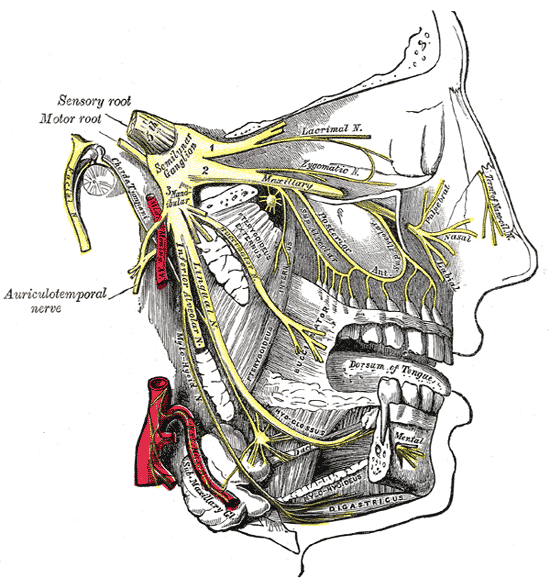
\includegraphics[width=120mm]{trig-branches.png}
 \centering
 \caption{Anatomy of the trigeminal nerve branches. \protect\cite{gray1918anatomy}} 
 \label{fig:trig-branches} 
 \end{figure}
 
Trigeminal sensory afferents include the myelinated A and unmyelinated C-fibres that originate from the subcutaneous sensory receptors responsible for mechano- and temperature pain, fine touch and vibration, such as the Messiner's, Pacinian and Ruffini corpuscles. 

The V1 branch provides the sensory innervation to the superior aspects of the face and cranium, including forehead, upper eyelids, eyeball, frontal sinus, lacrimal gland, and dura of the anterior cranial fossa. It further divides into lacrimal, frontal, and nasociliary nerve branches. The lacrimal branch supplies the lacrimal gland; the frontal contains smaller branches that innervate the skin of the medial forehead, upper eyelid, and parts of the frontal sinus; the nasociliary branch innervate various parts of the eye, and mucous membrane of the anterior nasal septum, anterior portion of the lateral nasal wall, and the skin on the tip of the nose. V1 exits the skullbase through the superior orbital fissure.  

The V2 provides innervation to the temple, cheek, lateral aspects of the nose, and lower eyelids via the zygomaticofacial and zygomaticotemporal branches. It also innervates upper oral cavity. It exits the skull through the foramen rotundum. 

V3 contains sensory and motor branches. It innervates skin of the jaw, areas above the ear, lips, gum, and teeth. The V3 division carries the mastication efferent to the four muscles recruited for mastications: the masseter, temporal, medial and lateral pterygoids. The tensor tympani also receives some CN V innervation, but it is primarily innervated by the facial nerve.  It is thought that CNV innervation is important in dampening the sound of chewing. V3 exits the skull through foramen ovale. 

The afferent branches converge and form the trigeminal ganglion (TRG) (also known as Gasserian, or semilunar ganglion), which then leads to the trunk or cisternal component of CN V. The TRG contains all the trigeminal sensory cell bodies. It situates in the Meckel's cave, in the middle cranial fossa. It is anatomically organized with respect to the trigeminal branches, with V1 situated in medial anterior, V2 in caudal lateral, and V3 in the middle.

The extension of the posterior aspect of the TRG forms the trigeminal nerve body, with both sensory and motor roots. The nerve body straddles the TRG and the trigeminal nucleus, by crossing the pontine cistern. The portion of the sensory nerve that enters the pons is termed the trigeminal root entry zone (REZ). The cistern trigeminal sensory nerve, similar to other peripheral nerves, is myelinated by Schwann cells. The myelin cell type transitions to oligodendrocyte myelinations in the CNS as it enters the pons. The CNS myelin can be several millimetres beyond the surface of the pons, before leading to the transition area, termed root entry zone, or Obersteiner-Redlich zone \cite{Peker2006}. A study in 100 CN V samples from 50 cadavers showed that cisternal CN V length ranges from 8-15 mm; the transition zone length is shorter on the medial aspect (0.1-2.5 mm) than the lateral aspect (0.17-6.75 mm). The transition zone can be up to 25\% of the nerve length \cite{Peker2006}. 

 \begin{figure}[h]
 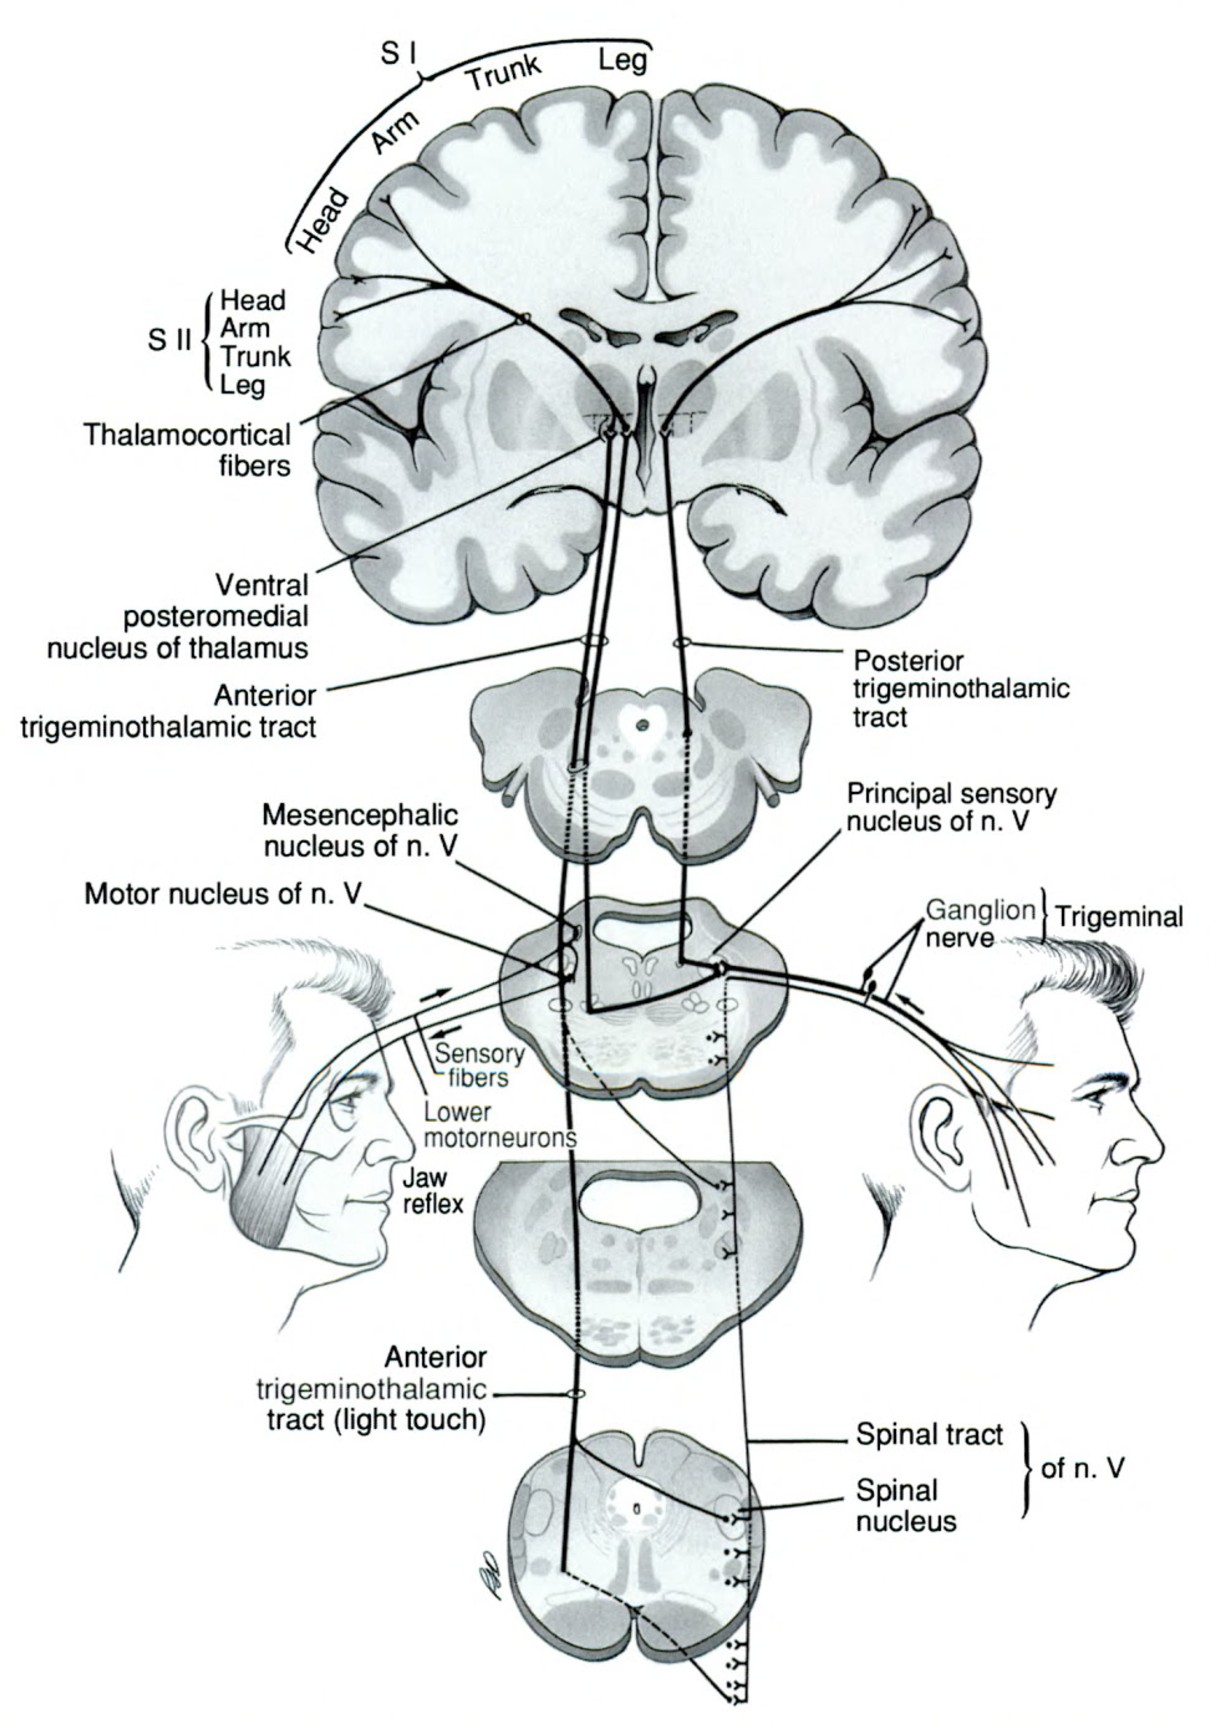
\includegraphics[width=105mm]{noback_2005_10_dot_6.jpg}
 \centering
 \caption{Overview of the trigeminal afferent pathways \protect\cite{noback2005human}. Reproduced with permission from Copyright Clearance Center (License ID: 4336271012841).}
 \label{fig:trig-pathway}
 \end{figure}
 
CN V passes into the pons (Figure \ref{fig:trig-pathway}), through the transverse pontine fibres and enters the tegmentum of the pontine brainstem. It then curve towards the medial aspect, and synapses onto the trigeminal nucleus in the basis of the pontine brainstem. The trigeminal brainstem sensory nucleus complex is divided, from superior to inferior, into the mesencephalic, main sensory, and spinal nuclei. The spinal nucleus can be further divided into pars oralis, pars interpolaris and pars caudalis. 

The mesencephalic nucleus is responsible for proprioception, while the spinal trigeminal nucleus receives ipsilateral pain and temperature afferents not only from CN V, but also from CN VII, CN IX and CN X. Pars oralis transmits fine tactile sensations from the oralfacial region, pars interpolaris is associated with dental pain, while pars caudalis is responsible for nociception and heat from the head. 

The main sensory nucleus receives discriminative input from the orofacial region, and along with the spinal trigeminal nucleus fibres, project to the contralateral ventral caudal nucleus (VC) of thalamus by decussating at various levels of the pons via the anterior trigeminothalamic tract. A separate branch responsible for oral cavity, however, projects to the ipsilateral VC via the dorsal trigeminothalamic tract.  

The VC thalamus projects to the primary sensory (S1) and secondary sensory (S2) cortical regions of the neocortex, thereby completing the afferent sensory projections of CN V. 



\subsection{Pathophysiology}

Classic TN is believed to be caused by neurovascular compression (NVC) of the CN V at its root entry zone (REZ) by the surrounding vasculature, where the nerve interfaces with the pons. An aberrant loop of artery and less commonly a vein is seen in 80-90\% of the cases of TN compressing the nerve \cite{Love2001,McLaughlin1999}. This can also be observed in conventional MR imaging \cite{Borges2010}. The superior cerebellar artery is responsible for most of the NVC (60-90\%), followed by the anterior inferior cerebellar artery (AICA) and basilar arteries \cite{Lutz2011}. There is a slight lateral prevalence, with right-sided TN occurring in  in 60\% of the cases, and in rare cases may be related to asymmetries of the foramen rotundum and foramen ovale \cite{Toda2009}.  Other types of compression may also cause TN; these can be in the forms of vestibular schwannomas, meningiomas, epidermoid cysts, and other cerebellopontine angle tumours, arteriovenous malformations and saccular aneurysms \cite{Haller2016,Love2001}. However NVC cannot be assumed to be directly causal of TN, since presence of vascular compression does not necessarily result in pain \cite{Desouza2013,Hodaie2013}. In approximately 10-15\% of cases where TN occurs with no observable vascular compression \cite{Revuelta-Gutierrez2006,Maarbjerg2015}.


Janetta \cite{Jannetta1967} proposed that NVC leads to focal demyelination of the trigeminal sensory root axons, and causes ephaptic nerve conductances that cause neuralgia. Ultrastructural examinations \cite{Love1998} of tissue samples obtained from CN V rhizotomy specimens showed oligodendrocyte demyelination at the site of root transition zone. Adjacent to the site of compression-related focal demyelination, thinly myelinated sheaths that encapsulate a number of demyelinated axons could be observed, suggesting aberrant remyelination. It is therefore plausible that NCV disrupts the central myelin. The region of disruption may include the peripheral-central myelin transition zone, and extending into central myelin regions.The TRG is also postulated to be responsible for neuralgia \cite{Rappaport1994}. It is believed that ganglionic ectopic firing can be triggered by mechanical disturbances as a result of nerve compression. Additionally, ganglionic cross action potential discharge may occur as a result of repeated stimulations in the nerve injury site, which ignites surrounding neurons. Histological findings by Devor et al. support the ignition hypothesis \cite{Devor2002a}, where demyelinated axons are shown to be in close apposition without intervening glia.  

\subsection{Treatment and outcomes}

The initial mode of treatment of TN consists in pharmacotherapy, primarily using anticonvulsant medication such as carbamazepine. While there is an initial, very good response to medical treatment, eventually nearly 50\% of patients will fail medical therapy, either due to side effects, or requirements of a progressive increase in dose \cite{Rappaport1994}. Multiple surgical treatments are available, from more central procedures addressing NVC to peripheral procedures such as neurectomy. The procedure that provides the greatest likelihood of pain relief is microvascular decompression (MVD) \cite{Lovely1997,Hodaie2013}, where the nerve is decompressed from the offending vascular structure through the placement of a piece of Teflon\textcopyright gauze. This is thought to dampen the pulsations of the artery on the nerve. MVD can result in 90\% pain relief immediately after surgery \cite{Zakrzewska2005}, and a long-term success rate of 70\% at 10 years \cite{Barker1996}.
Partial sensory rhizotomy (PSR) can also be performed, where the offending CN V branch is severed, with a response rate of 88-70\% \cite{Young1993,Zakrzewska2005}. 

Intervention can also be non-invasive, in the form of Gamma Knife radiosurgery (GKRS) \cite{Hodaie2012g}. The Perfexion GK system focuses gamma radiation from 192 cobalt-60 ($^{60}$Co) sources onto specific targets along the trigeminal nerve. The target is either on the cisternal segment of CN V or just outside of the REZ \cite{Daugherty2015}. Proximal targets correlate with longer pain relief, but also higher chance of facial numbness\cite{Xu2014}. The procedure requires a stereotactic frame, and a dose of 70-90 Gy delivered to the nerve. The effect is delayed and pain relief can be experienced in 4-6 weeks post-radiosurgery. GKRS treatments result in 75\% initial pain relief \cite{Tuleasca2015,Kondziolka2010}, about 50-80\% remain pain-free at 1 year, 45-65\% 2 years and 30-40\% 3 years after surgery \cite{Kondziolka2010,Sheehan2005}. Better treatment outcomes were related to factors such as having no other accompanying symptoms, no prior surgery and shorter term pain history of fewer than three years.

\subsection{Neuroimaging of Trigeminal Neuralgia}

Neuroimaging of the TN has been challenging, due to the small diameter of the CN V and since the contrast of the CNS trigeminal pathways is difficult to distinguish from the surrounding on conventional MRI \cite{Borges2010}. In conventional MRI, the brainstem nerve segment can only be deduced from its surrounding structures \cite{Casselman2008}. Sequences that can visualize myelinated structures are chosen, these include T2-weighted MRI  sequences such as FIESTA and CISS. Manual segmentation of T1 and T2 MRI requires great effort, with mixed results \cite{Miller2008a}. Diffusion MRI provided fibre orientation, and early attempts to segment the trigeminal system showed promise \cite{Upadhyay2008,Habas2007f}. Additionally, DTI showed strong ability to visualize spatial relationships in white matter anatomy, for example in delineating fornix sub-regions \cite{Chen2015c}, and in visualizing the distortion of CN VII/VIII by vestibular schwannomas \cite{Chen2011b}.  

Tractography allows high quality \textit{in-vivo} reconstructions of human cranial nerves \cite{Hodaie2010}. Cisternal CN V could be reliably delineated with Gaussian tensors with just 25 MR gradient directions. This permitted high fidelity visualization and targeted characterization of CN V diffusivity in TN, demonstrating significant reduction in fractional anisotropy (FA) post-surgery at the site of the GK target \cite{Hodaie2009a}. Study of CN V diffusivity in conjunction with deep white matter again revealed reduced FA on the affected CN V, with also bilateral increased in radial, axial, and mean diffusivity. Disruptions were also found in the cognitive-affective, attention, and motor regions of the cortex, consistent with cortical patterns in chronic pain \cite{Desouza2013}. Lowered FA was reported in multiple TN studies \cite{Herweh2007, Lutz2011}. A study in patients with temporomandibular disorder (TMD) showed a bilateral reduction in CN V FA compared to controls, with the FA of the affected side significantly inverse-correlates with pain duration \cite{Moayedi2012}. This TMD study also revealed similar cognitive and motor disruption, and internal capsule FA significantly inverse-correlated with pain intensity. 